% Week 4 report -- compile from this folder: pdflatex report_week4.tex
% Figures and tables are read directly from 03_output/week4/ (built by 02_analysis/02_week4_trees.py)
\documentclass[11pt]{article}
\usepackage[margin=0.8in]{geometry}
\usepackage{graphicx,booktabs,float,amsmath}
\usepackage[font=small,labelfont=bf,skip=3pt]{caption}
\setlength{\parindent}{0pt}
\setlength{\parskip}{4pt}
\pagestyle{empty}
\graphicspath{{../}}

\begin{document}

\begin{center}
{\large\bfseries Do Local Chiefs Grant More Favors? Collector Type, Tax Exemptions and Bribery in Kananga}\\[3pt]
Name: Tsu Ning Tsao \qquad Student Number: 1012713137
\end{center}
\vspace{-6pt}

\textbf{Set-up.} Neighbourhoods were randomly assigned to chief (Local) or state (Central) collection, so Local$-$Central differences are causal. With stratum fixed effects and SEs clustered by neighbourhood (14,381 properties, 221 neighbourhoods), Local raises the share exempted from 26.4\% to about 30.4\% ($+4.0$ pp, SE 2.0). The increase is driven by old age ($+3.5$ pp, SE 1.4); widow exemptions do not move ($-0.1$ pp, SE 1.2) and reported bribes are unchanged ($+0.2$ pp on a 1.4\% base, SE 0.3). Old-age exemptions given to owners whom our survey records as under 60 rise from 2.2\% to 3.6\% ($+1.4$ pp, SE 0.6), a first measure of discretionary exemptions. Below, $Y=\texttt{exempt}$ is predicted for the 6,292 properties with surveyed owner age and sex, using 16 pre-treatment features; train/test is an 80/20 split by neighbourhood (163/41) and all tuning uses 10-fold CV grouped by neighbourhood inside the training set.

\section*{1. Regression Tree Visualization}
\vspace{-6pt}
\begin{figure}[H]
\centering
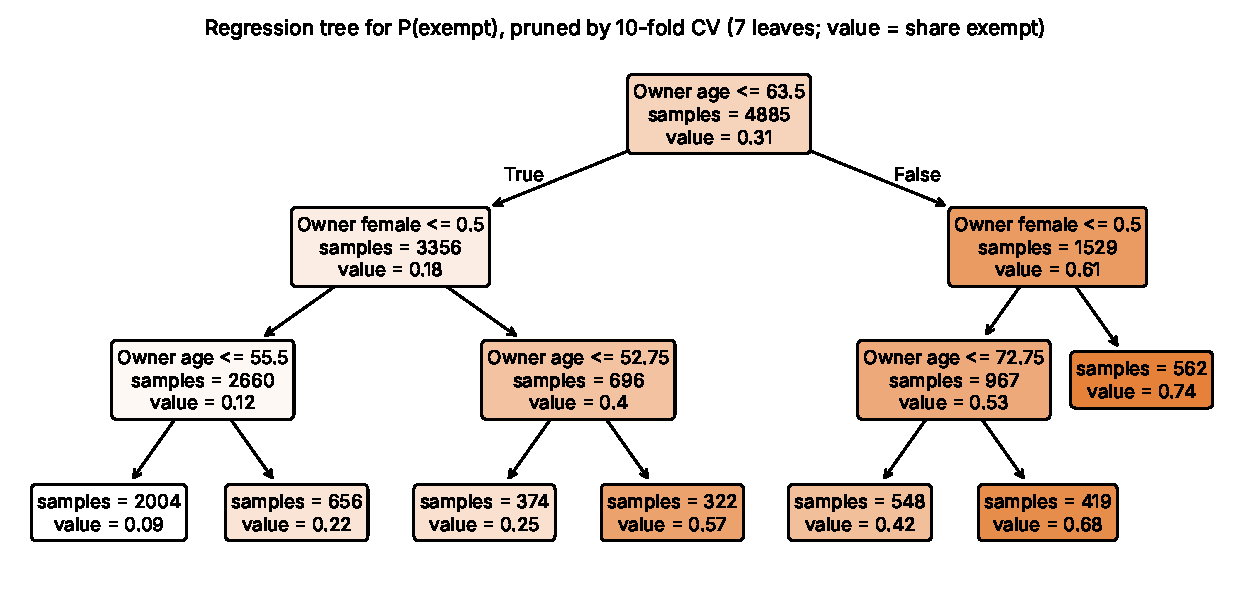
\includegraphics[width=0.92\textwidth]{figure_w4_1_regression_tree.pdf}
\caption{Pruned regression tree for $P(\text{exempt})$; $\alpha$ chosen by grouped 10-fold CV (7 leaves, depth 3). ``Owner female $\le 0.5$'' (left branch) means male owner.}
\end{figure}
\vspace{-8pt}
The tree splits only on owner age and sex: exemption rises from 9\% (men $\le$55) to 74\% (women over 63.5). It never splits on Local, although OLS finds a significant $+4$ pp effect, because a 4 pp shift is small next to these 60-point age and sex gaps; a prediction tree ranks variables by how much they explain $Y$, not by causal importance, so it is the wrong tool for finding where Local matters. What the tree adds over OLS is the shape of the exemption rule. Women are exempted from about 53 (57\% vs 25\% below), consistent with widowhood rather than age, and 22\% of men aged 55--63 are exempted, many of them below a 60-year old-age threshold. That leaf is where discretionary ``old-age'' exemptions live, which tells me to estimate heterogeneity in the Local effect by age around the cutoff in later weeks.

\section*{2. Random Forest Importance Matrix}
\vspace{-6pt}
\begin{figure}[H]
\centering
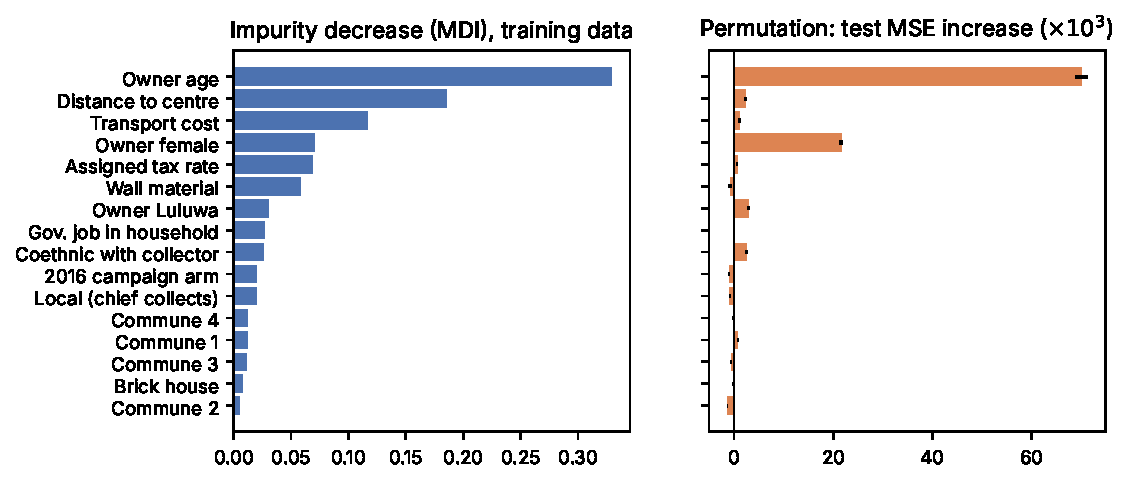
\includegraphics[width=0.86\textwidth]{figure_w4_2_rf_importance.pdf}
\caption{Random forest ($m=5$, 500 trees). Left: mean decrease in impurity on training data. Right: increase in test MSE when a feature is permuted (20 repeats, $\pm$1 SE). Full values in \texttt{table\_w4\_2\_rf\_importance.csv}.}
\end{figure}
\vspace{-8pt}
Owner age is the most influential feature on both measures, followed by owner sex on the permutation measure. Distance to the centre and transport cost rank 2nd and 3rd by impurity but barely raise test error when permuted, the known bias of impurity importance towards continuous features with many split points; Local is near zero on both, as in the tree.

\section*{3. Error Comparison for Bagging, Boosting, Tree, and Random Forest}
\vspace{-4pt}
\begin{table}[H]
\centering\small
\begin{tabular}{lcccc}
\hline
Model & Test MSE & Test RMSE & \% vs mean & OOB MSE \\
\hline
Mean only (benchmark) & 0.2048 & 0.4525 & +0.0 & -- \\
OLS (linear probability) & 0.1428 & 0.3780 & -30.2 & -- \\
Regression tree (pruned) & 0.1434 & 0.3786 & -30.0 & -- \\
Bagging (m = p = 16) & 0.1553 & 0.3941 & -24.2 & 0.1546 \\
Random forest (m = 5) & 0.1490 & 0.3860 & -27.2 & 0.1486 \\
Boosting (B = 272, $\lambda$ = 0.01, d = 3) & 0.1412 & 0.3758 & -31.0 & -- \\
\hline
\end{tabular}

\caption{Test error on the 1,407 held-out properties (41 neighbourhoods). MSE of a 0/1 outcome is the Brier score. The boosting iteration count was chosen by grouped CV on the training set, not on the test set. OOB MSE is on the training set.}
\end{table}
\vspace{-8pt}
Boosting has the lowest test MSE (0.141), but OLS (0.143) and the 7-leaf tree (0.143) are within 2\%, and all improve on the mean by about 30\%. The gain comes almost entirely from owner age and sex, a structure simple enough for a small tree. Bagging is the worst model (0.155): its unpruned trees all split first on age, so they are highly correlated and averaging removes little of their variance. The random forest, which decorrelates trees by sampling $m=5$ features at each split, closes about half of that gap, and the OOB errors match the test errors closely.

\end{document}
